% GENERATED by make_paper_assets.py -- do not edit by hand.
\begin{figure}[t]
\centering
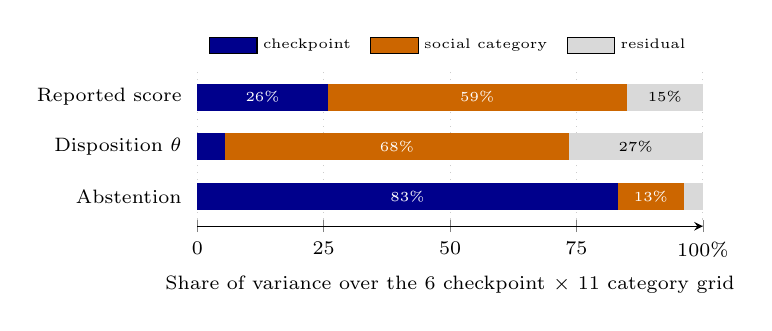
\begin{tikzpicture}
\begin{axis}[
  width=0.66\columnwidth, height=3.6cm, xmin=0, xmax=100, ymin=0.4, ymax=3.6,
  legend columns=3, legend style={at={(0.5,1.02)}, anchor=south, draw=none, font=\tiny,
    /tikz/every even column/.append style={column sep=5pt}},
  xtick={0,25,50,75,100}, xticklabels={0,25,50,75,100\%},
  ytick={1,2,3}, yticklabels={Abstention,Disposition $\theta$,Reported score},
  tick label style={font=\scriptsize}, label style={font=\scriptsize},
  xlabel={Share of variance over the 6 checkpoint $\times$ 11 category grid},
  axis lines=left, y axis line style={draw=none}, ytick style={draw=none},
  xmajorgrids, grid style={dotted, gray!40}, clip=false,
]
\fill[blue!55!black] (axis cs:0.00,2.73) rectangle (axis cs:25.83,3.27);
\node[font=\tiny, text=white] at (axis cs:12.91,3) {26\%};
\fill[orange!80!black] (axis cs:25.83,2.73) rectangle (axis cs:84.92,3.27);
\node[font=\tiny, text=white] at (axis cs:55.37,3) {59\%};
\fill[gray!30] (axis cs:84.92,2.73) rectangle (axis cs:100.00,3.27);
\node[font=\tiny, text=black] at (axis cs:92.46,3) {15\%};
\fill[blue!55!black] (axis cs:0.00,1.73) rectangle (axis cs:5.57,2.27);
\fill[orange!80!black] (axis cs:5.57,1.73) rectangle (axis cs:73.43,2.27);
\node[font=\tiny, text=white] at (axis cs:39.50,2) {68\%};
\fill[gray!30] (axis cs:73.43,1.73) rectangle (axis cs:100.00,2.27);
\node[font=\tiny, text=black] at (axis cs:86.72,2) {27\%};
\fill[blue!55!black] (axis cs:0.00,0.73) rectangle (axis cs:83.14,1.27);
\node[font=\tiny, text=white] at (axis cs:41.57,1) {83\%};
\fill[orange!80!black] (axis cs:83.14,0.73) rectangle (axis cs:96.29,1.27);
\node[font=\tiny, text=white] at (axis cs:89.72,1) {13\%};
\fill[gray!30] (axis cs:96.29,0.73) rectangle (axis cs:100.00,1.27);
\addlegendimage{area legend, draw=none, fill=blue!55!black}
\addlegendentry{checkpoint}
\addlegendimage{area legend, draw=none, fill=orange!80!black}
\addlegendentry{social category}
\addlegendimage{area legend, draw=none, fill=gray!30}
\addlegendentry{residual}
\end{axis}
\end{tikzpicture}
\caption{Where the variance lives. In the evaluated grid, abstention varies mainly by
checkpoint, while the stereotype-aligned rate $\theta$ varies mainly by social
category. The reported score $s_{\text{AMB}}=(1-\text{abstention})\cdot b$ mixes
both, so comparing \emph{checkpoints} ranks them substantially by abstention, while
comparing \emph{categories} within a checkpoint tracks disposition. (Additive two-way
decomposition. The residual is interaction plus sampling noise.)}
\label{fig:variance}
\end{figure}
